\documentclass[pscyr]{hedlab}
\usepackage[russian]{babel}
\usepackage{graphicx}
\graphicspath{{images/}}
\usepackage{listings}

\lstset{
  basicstyle=\footnotesize,
  inputencoding=utf8,
  extendedchars=True,
  language=[Sharp]C,
  numbers=left,
  numberstyle=\footnotesize,
  breakatwhitespace=\false,
  breaklines=True,
  tabsize=2,
  keepspaces=true,
}

\labname{Публикация данных в веб\\Вариант 1}
\labnum{3}
\student{Голубев~А.~В., САПР-1.1п}
\labdate{}

\begin{document}

  \makeheader

  \emph{Цель:} получение практических навыков создания базы данных СУБД
  Microsoft SQL Server Express посредством Microsoft Visual Studio и
  получения информации из таблиц базы данных в веб-приложении.
  
  \emph{Задание:}
  \begin{itemize}
    \itemsep -5pt
    \item создайте базу данных со структурой таблиц, указанной для
      соответствующего варианта;
    \item заполните таблицы не менее чем на 15 записей;
    \item создайте веб-сайт с веб-формами: для каждой таблицы создайте
      отдельную веб-форму, на которой отобразите содержимое таблицы.

  \end{itemize}
  
  Реализовать механизм передачи информации между страницами с использованием
  переменной сессии.

  \emph{Выполнение лабораторной работы:}
  В качестве исходных данных выступает структура базы данных, приведенная на
  рисунке~\ref{pic:1},
  \begin{figure}[h!]
    \vspace{-1em}\center
    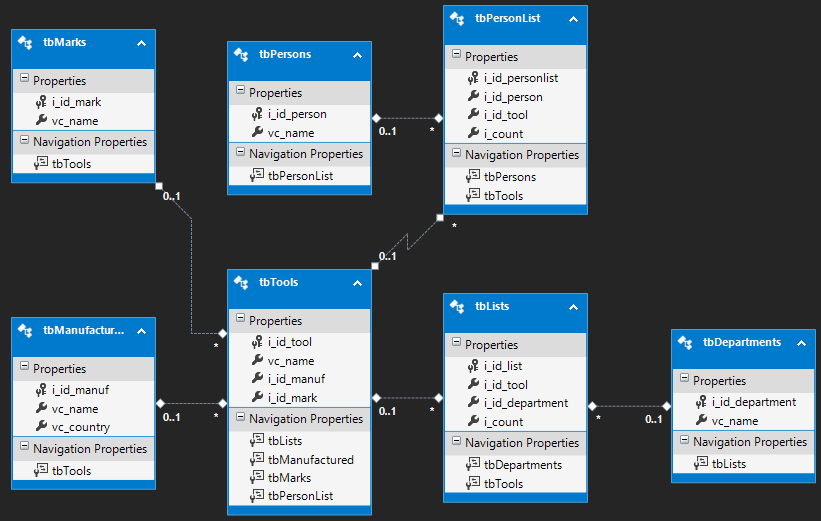
\includegraphics[width=.95\textwidth]{structure}
    \caption{Структура базы данных}
    \label{pic:1}
  \end{figure}
  
  где таблицы имеют следующую структуру:
  \begin{table}[h!]
    \caption{таблица tbDepartments}
    \vspace{-1em}\center
    \begin{tabular}{|C{.06}|*{2}{C{.15}|}C{.3}|} \hline
      № п/п & Наименование поля & Тип & Примечание \\ \hline
      1 & i\_id\_department & Int & Primary key;
        Identity = Yes; Indentity seed = 1; Indentity~Increment~=~1 \\ \hline
      2 & vc\_name & Varchar(50) & \\ \hline
    \end{tabular}
  \end{table}
  
  \begin{table}[h!]
    \caption{таблица tbTools}
    \vspace{-1em}\center
    \begin{tabular}{|C{.06}|*{2}{C{.15}|}C{.3}|} \hline
      № п/п & Наименование поля & Тип & Примечание \\ \hline
      1 & i\_id\_tool & Int & Primary key;
        Identity = Yes; Indentity seed = 1; Indentity~Increment~=~1 \\ \hline
      2 & vc\_name & Varchar(50) & Not Null;
        Default value = 'Неизвестный'\\ \hline
      3 & i\_id\_manuf & Int & Внешний ключ,
        ссылка на таблицу~tbManufactured \\ \hline
      4 & i\_id\_mark & Int & Внешний ключ,
        ссылка на таблицу~tbMarks \\ \hline
    \end{tabular}
  \end{table}
  
  \begin{table}[h!]
    \caption{таблица tbPersons}
    \vspace{-1em}\center
    \begin{tabular}{|C{.06}|*{2}{C{.15}|}C{.3}|} \hline
      № п/п & Наименование поля & Тип & Примечание \\ \hline
      1 & i\_id\_person & Int & Primary key;
        Identity = Yes; Indentity seed = 1; Indentity~Increment~=~1 \\ \hline
      2 & vc\_name & Varchar(50) & Not Null;
        Default value = 'Иванов~Иван~Иванович'\\ \hline
    \end{tabular}
  \end{table}

  \clearpage
  
  \begin{table}[h!]
    \caption{таблица tbPersonList}
    \vspace{-1em}\center
    \begin{tabular}{|C{.06}|*{2}{C{.15}|}C{.3}|} \hline
      № п/п & Наименование поля & Тип & Примечание \\ \hline
      1 & i\_id\_personlist & Int & Primary key;
        Identity = Yes; Indentity seed = 1; Indentity~Increment~=~1 \\ \hline
      2 & i\_id\_person & Int & Внешний ключ,
        ссылка на таблицу~tbPersons \\ \hline
      3 & i\_id\_tool & Int & Внешний ключ,
        ссылка на таблицу~tbTools \\ \hline
      4 & i\_count & Int & Not Null, Default value = 0 \\ \hline
    \end{tabular}
  \end{table}
  
  \begin{table}[h!]
    \caption{таблица tbMarks}
    \vspace{-1em}\center
    \begin{tabular}{|C{.06}|*{2}{C{.15}|}C{.3}|} \hline
      № п/п & Наименование поля & Тип & Примечание \\ \hline
      1 & i\_id\_mark & Int & Primary key;
        Identity = Yes; Indentity seed = 1; Indentity~Increment~=~1 \\ \hline
      2 & vc\_name & Varchar(50) & Not Null;
        Default value = 'Марка' \\ \hline
    \end{tabular}
  \end{table}
  
  \clearpage
  
  \begin{table}[h!]
    \caption{таблица tbManufactured}
    \vspace{-1em}\center
    \begin{tabular}{|C{.06}|*{2}{C{.15}|}C{.3}|} \hline
      № п/п & Наименование поля & Тип & Примечание \\ \hline
      1 & i\_id\_manuf & Int & Primary key;
        Identity = Yes; Indentity seed = 1; Indentity~Increment~=~1 \\ \hline
      2 & vc\_name & Varchar(50) & Not Null;
        Default value = 'Производитель' \\ \hline
      3 & vc\_country & Varchar(50) & Not Null;
        Default value = 'Россия' \\ \hline
    \end{tabular}
  \end{table}
  
  \begin{table}[h!]
    \caption{таблица tbLists}
    \vspace{-1em}\center
    \begin{tabular}{|C{.06}|*{2}{C{.15}|}C{.3}|} \hline
      № п/п & Наименование поля & Тип & Примечание \\ \hline
      1 & i\_id\_list & Int & Primary key;
        Identity = Yes; Indentity seed = 1; Indentity~Increment~=~1 \\ \hline
      2 & i\_id\_tool & Int & Внешний ключ,
        ссылка на таблицу~tbTools \\ \hline
      3 & i\_id\_department & Int & Внешний ключ,
        ссылка на таблицу~tbDepartments \\ \hline
      4 & i\_count & Int & Not Null, Default value = 0 \\ \hline
    \end{tabular}
  \end{table}
  
  Скриншоты страниц:
  \begin{figure}[h!]
    \center
    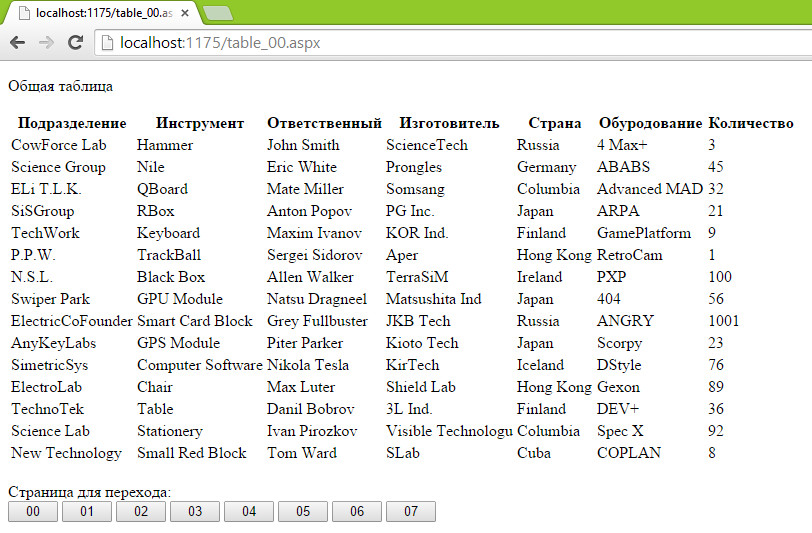
\includegraphics[width=.8\textwidth]{lab03_01}
    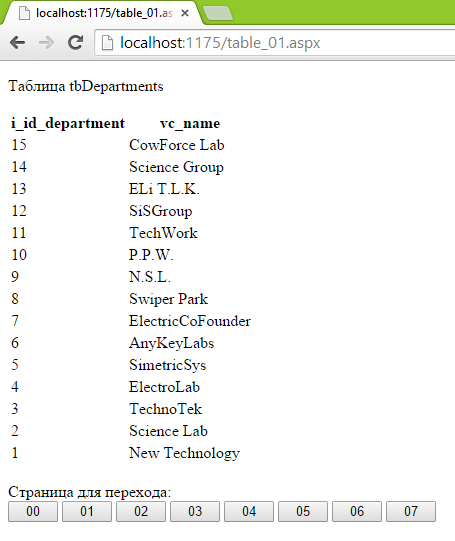
\includegraphics[width=.47\textwidth]{lab03_02} \hspace{1em}
    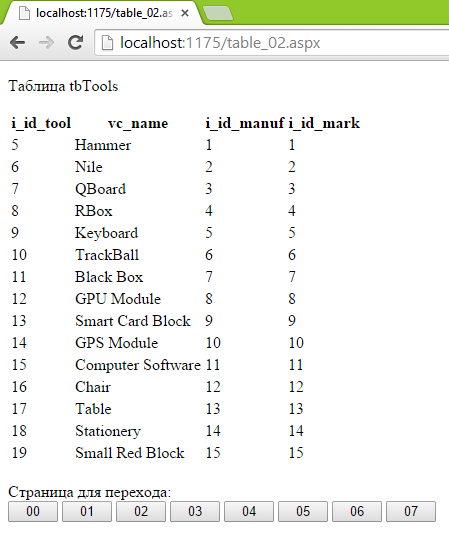
\includegraphics[width=.47\textwidth]{lab03_03}
  \end{figure}
  \begin{figure}[h!]
    \center
    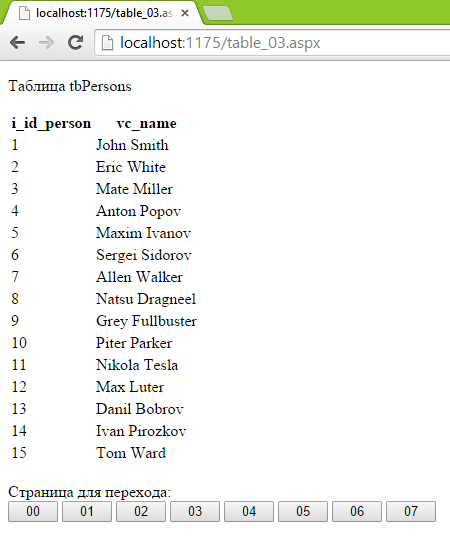
\includegraphics[width=.47\textwidth]{lab03_04} \hspace{1em}
    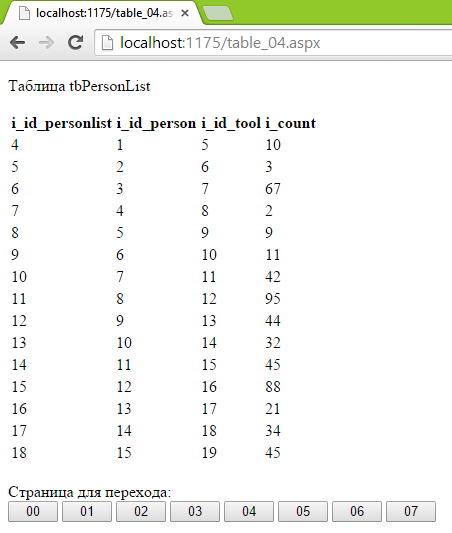
\includegraphics[width=.47\textwidth]{lab03_05} \\
    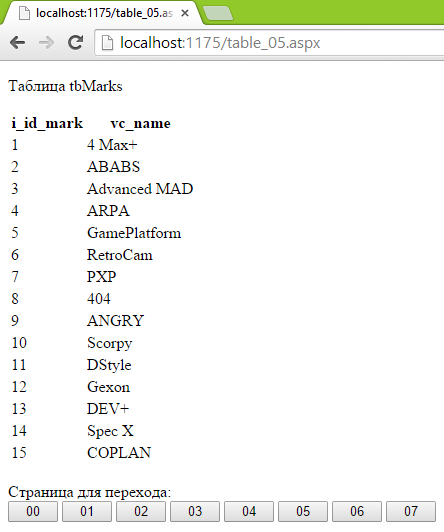
\includegraphics[width=.47\textwidth]{lab03_06} \hspace{1em}
    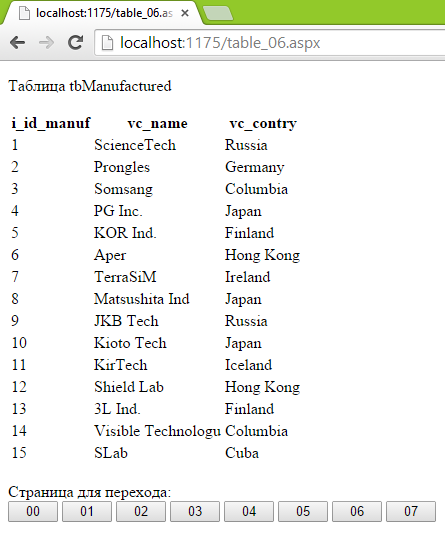
\includegraphics[width=.47\textwidth]{lab03_07}
  \end{figure}
  \begin{figure}[h!]
    \center
    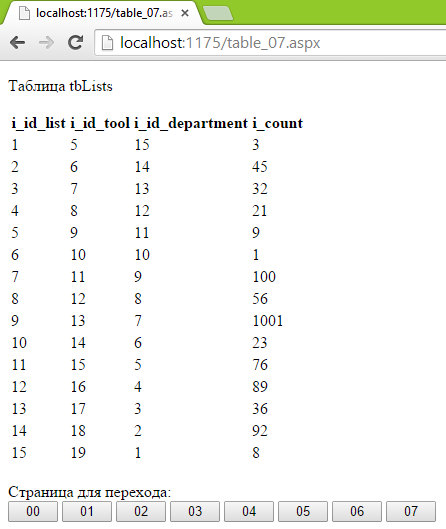
\includegraphics[width=.47\textwidth]{lab03_08}
  \end{figure}
  \clearpage
  
  Пример кода страницы и классов кода страницы \textbf{table\_00.aspx}:
  \lstinputlisting[inputencoding=koi8-r,language=HTML]{./code/lab03_table_00.aspx}
  
  \vspace{2em}
  \textbf{table\_00.aspx.cs}:
  \lstinputlisting{./code/lab03_table_00.aspx.cs}
  
  \emph{Вывод:} в результате проделанной работы
  \vspace{-.5em}  
  \begin{enumerate}
    \itemsep -5pt
    \item создал проект веб-сайта;
    \item создал базу данных, таблицы базы данных согласно заданию и
      наполнил таблицы информацией;
    \item создал объект SQLDataSource и настроил его на получение информации
      из связанных таблиц;
    \item реализовал метод получения данных из таблиц и отображения их на
      странице веб-сайта.
  \end{enumerate}

\end{document}